\section{Persistencia}
\label{sec:persistencia}

Una estructura de datos se dice \textit{persistente} si preserva sus estados anteriores, incluso después de realizarle actualizaciones.
En lugar de modificar los valores almacenados en cada nodo, lo que vamos a hacer es crear ``clones'' de los nodos a cambiar, con las modificaciones necesarias ya aplicadas.
De esta forma, como no se modificó ningún valor, no se invalida una representación vieja al hacer actualizaciones.

En el caso del Treap, sólo vamos a crear \(\mathcal{O}(\lg n)\) nodos adicionales por llamado a Split() / Merge(), y es cuestión de reemplazar asignaciones por crear nodos nuevos.

Detalle de implementación: como puede ser difícil llevar cuenta de qué punteros tenemos que borrar en cada momento,
es conveniente usar punteros inteligentes (\texttt{std::shared\_ptr}), para que la memoria se libere cuando no es usada.

\begin{minted}{c++}
pair<Treap, Treap> split(Treap root, int k) {
 if (root == nullptr) return {nullptr, nullptr};

 Treap left, right;
 if (root->key <= k) {
  left = make_shared<Node>(*root);
  tie(left->right, right) = split(root->right, k);
  evaluate(left);
 } else {
  right = make_shared<Node>(*root);
  tie(left, right->left) = split(root->left, k);
  evaluate(right);
 }
 return {left, right};
}

Treap merge(Treap left, Treap right) {
 if (left == nullptr) return right;
 if (right == nullptr) return left;

 Treap root;
 if (left->priority > right->priority) {
  root = make_shared<Node>(*left);
  root->right = merge(left->right, right);
 } else {
  root = make_shared<Node>(*right);
  root->left = merge(left, right->left);
 }
 evaluate(root);
 return root;
}
\end{minted}

Persistencia todavía no es un tema común en competencias, y menos todavía Treaps Persistentes.
Sin embargo, nos permite hacer en \(\mathcal{O}(\lg n)\) operaciones que la intuición dice no deberían ser posibles, como llamar a Merge() de parte de un árbol con sí mismo,
usando otro truco conocido como ``Treap con Prioridades Implícitas''.

\subsection{SWERC 2020 - H. Figurines}
\problema{
\textbf{H. Figurines:} (resumido)

Tenemos un conjunto, inicialmente vacío, y los números \(1, \dots n\).
A lo largo de \(n\) días, vamos a insertar y eliminar estos números, cada uno exáctamente una vez.

Responder \(q\) consultas, del tipo ``¿Cuántos elementos mayores o iguales que \(x\) había en el conjunto, al finalizar el día \(d\)?''.

\url{https://codeforces.com/gym/103081/problem/H}
}

La solución al problema es usar un \hyperref[sec:order-statistics-tree]{Order Statistics Tree} Persistente para resolver el problema.
Primero, queremos generar los \(n\) árboles, insertando y removiendo del árbol apropiado.
Luego, es cuestión de procesar las consultas en orden, llamando a Rank() en el Treap con índice \(d\).

Nota: esta versión resumida del problema puede resolverse sin usar persistencia, pues podemos ordenar las consultas por día, de manera que sólo hay un árbol activo a la vez.
En el problema original esto no es posible, porque el valor \(x\) de cada consulta depende de la respuesta a la consulta anterior.

\subsection{CodeChef - GENETICS}
\problema{
\textbf{GENETICS:}

Tenemos \(n\) cadenas de ADN \(D_1, \dots D_n\) (palabras con letras A, C, G, T),
y podemos realizar tres tipos de operaciones sobre las mismas:

\begin{enumerate}
\item Combinar(\(i_1, i_2, k_1, k_2\)): 

Añade las cadenas \(D_{i_1}[1 .. k_1] + D_{i_2}[k_2+1 ..]\) y \(D_{i_2}[1 .. k_2] + D_{i_1}[k_1+1..]\) al final de la lista

\item Mutar(\(i, k, c\)): Cambia el carácter en la posición \(k\) de \(D_i\) por \(c\)
\item Contar(\(i, l, r\)): Devuelve la frecuencia de cada carácter en \(D_i[l..r]\)
\end{enumerate}

Se garantiza que no se van a producir cadenas de longitud mayor a \(2 \cdot 10^9\).

\url{https://www.codechef.com/problems/GENETICS}
}

Notar que la cota sobre la longitud máxima es importante, porque podemos duplicar el tamaño de la cadena más larga en un paso con un llamado a Combinar().

\begin{center}
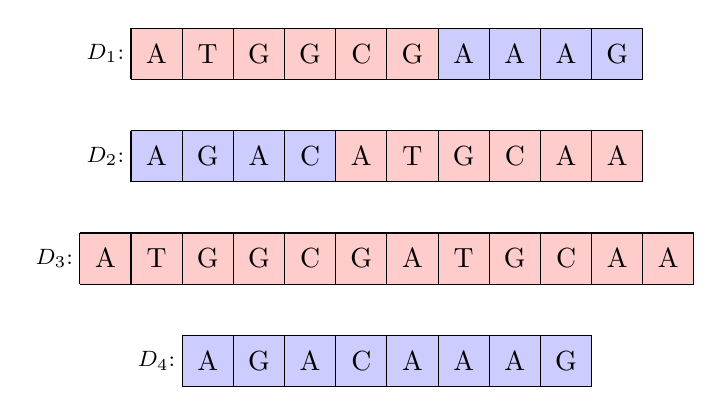
\begin{tikzpicture}[xscale=0.65, yscale=-0.65]

\normalsize
\fill[red!20](0,0) rectangle (6, 1);
\fill[blue!20](6,0) rectangle (10, 1);
\draw (0,0) grid (10,1);
\node at (0.5,0.5) {A};
\node at (1.5,0.5) {T};
\node at (2.5,0.5) {G};
\node at (3.5,0.5) {G};
\node at (4.5,0.5) {C};
\node at (5.5,0.5) {G};
\node at (6.5,0.5) {A};
\node at (7.5,0.5) {A};
\node at (8.5,0.5) {A};
\node at (9.5,0.5) {G};

\footnotesize
\node at (-0.5,0.5) {$D_1$:};

\normalsize
\fill[blue!20](0,2) rectangle (4, 3);
\fill[red!20](4,2) rectangle (10, 3);
\draw (0,2) grid (10,3);
\node at (0.5,2.5) {A};
\node at (1.5,2.5) {G};
\node at (2.5,2.5) {A};
\node at (3.5,2.5) {C};
\node at (4.5,2.5) {A};
\node at (5.5,2.5) {T};
\node at (6.5,2.5) {G};
\node at (7.5,2.5) {C};
\node at (8.5,2.5) {A};
\node at (9.5,2.5) {A};

\footnotesize
\node at (-0.5,2.5) {$D_2$:};

\normalsize
\fill[red!20](-1,4) rectangle (11, 5);
\draw (-1, 4) grid (11, 5);
\node at (-0.5,4.5) {A};
\node at (0.5,4.5) {T};
\node at (1.5,4.5) {G};
\node at (2.5,4.5) {G};
\node at (3.5,4.5) {C};
\node at (4.5,4.5) {G};
\node at (5.5,4.5) {A};
\node at (6.5,4.5) {T};
\node at (7.5,4.5) {G};
\node at (8.5,4.5) {C};
\node at (9.5,4.5) {A};
\node at (10.5,4.5) {A};

\footnotesize
\node at (-1.5, 4.5) {$D_3$:};

\normalsize
\fill[blue!20](1,6) rectangle (9, 7);
\draw (1, 6) grid (9, 7);
\node at (1.5,6.5) {A};
\node at (2.5,6.5) {G};
\node at (3.5,6.5) {A};
\node at (4.5,6.5) {C};
\node at (5.5,6.5) {A};
\node at (6.5,6.5) {A};
\node at (7.5,6.5) {A};
\node at (8.5,6.5) {G};

\footnotesize
\node at (0.5, 6.5) {$D_4$:};
\end{tikzpicture}
\captionof{figure}{Ejemplo de Combinar()}
\end{center}

Del diagrama podemos ver que Combinar() es cortar en dos las cadenas originales, y pegarlas para obtener una cadena nueva.
Por esta razón, vamos a representar cada cadena con un Treap Persistente con claves implícitas, y procedemos de la forma que muestra el diagrama.

Para hacer los llamados a Mutar(), vamos a sobrescribir la posición en la lista de cadenas
con el resultado de sacar el nodo viejo en la posición \(k\), e insertar el nuevo.
No podemos modificar directamente el nodo, porque podrían verse afectadas otras cadenas que apunten a ese nodo o algún antecesor.

Para los llamados a Contar(), mantenemos en cada nodo como función acumulada una tupla, que representa la frecuencia de cada carácter, 
y obtener la respuesta es igual que otros problemas de Range Queries.

Por lo tanto, la complejidad temporal es \(\mathcal{O}(n |s| + q \lg L)\), donde \(|s|\) es la longitud máxima de una cadena del input (en este caso, 30000), 
y \(L\) es la longitud máxima que puede tener una cadena.

\subsection{Petrozavodsk Summer Training Camp 2017 - C. Sequence}

\problema{
\textbf{C. Sequence:}

Tenemos un array \(A = a_1 \dots a_n\), y tres tipos de operaciones:
\begin{enumerate}
\item Computar la suma en el rango \([l, r]\)
\item Correr el siguiente pseudocódigo:

\texttt{for (l <= i <= r) a[i] = a[i - k];}
\item Asignar \(a_i = a'_i\) para todo \(i \in [l, r]\)
\end{enumerate}

Donde \(A' = a'_1 \dots a'_n\) son los valores originales de \(A\).

\url{https://www.acmicpc.net/problem/19068}
}

Vamos a usar un Treap con claves implícitas para mantener las sumas de rangos, queremos ver cómo soportar las otras dos operaciones.
Además, necesitamos un cierto nivel de persistencia, pero en un momento dado sólo nos interesan dos árboles: el original, y el actual.

Las operaciones de tipo 3. son relativamente simples, tenemos que usar Split() para conseguir el rango [l, r] del árbol original, y reemplazarlo en el Treap actual:

\begin{minted}{c++}
Treap toCopy 
  = split(split(orig, r).first, l - 1).second;
auto [left, right] = split(root, r);
left = split(left, l - 1).first;
root = merge(merge(left, toCopy), right);
\end{minted}

El verdadero problema son las operaciones de tipo 2., que no es inmediato ver como evitar correr el pseudocódigo. 
Esto se debe a que, como los rangos de inicio y llegada pueden intersecarse, no es necesariamente reemplazar el rango \([l - k, r - k]\) en la posición \([l, r]\).

\begin{center}
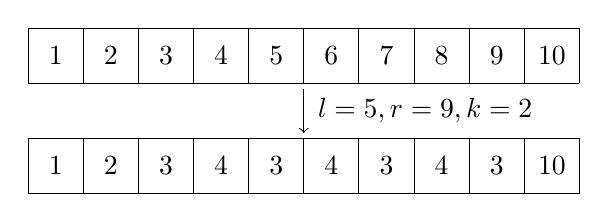
\begin{tikzpicture}[xscale=0.7, yscale=-0.7]

\draw (0,0) grid (10,1);
\node at (0.5,0.5) {$1$};
\node at (1.5,0.5) {$2$};
\node at (2.5,0.5) {$3$};
\node at (3.5,0.5) {$4$};
\node at (4.5,0.5) {$5$};
\node at (5.5,0.5) {$6$};
\node at (6.5,0.5) {$7$};
\node at (7.5,0.5) {$8$};
\node at (8.5,0.5) {$9$};
\node at (9.5,0.5) {$10$};

\draw[arrows={->}] (5, 1.1) -- (5, 1.9);
\node at (7.2, 1.5) {$l = 5, r = 9, k = 2$};

\draw (0,2) grid (10,3);
\node at (0.5,2.5) {$1$};
\node at (1.5,2.5) {$2$};
\node at (2.5,2.5) {$3$};
\node at (3.5,2.5) {$4$};
\node at (4.5,2.5) {$3$};
\node at (5.5,2.5) {$4$};
\node at (6.5,2.5) {$3$};
\node at (7.5,2.5) {$4$};
\node at (8.5,2.5) {$3$};
\node at (9.5,2.5) {$10$};

\end{tikzpicture}
\captionof{figure}{Ejemplo de operación tipo 2}
\end{center}

Luego de observar un par de ejemplos, podemos ver que estamos repitiendo el rango \([l - k, l - 1]\) varias veces, y colocándolo en el rango \([l, r]\).
Podemos duplicar la longitud del rango con cada llamado a Merge(), y cada llamado cuesta \(\mathcal{O}(\lg n)\), entonces podemos responder estas consultas en \(\mathcal{O}(\lg^2 n)\).

Hay un pequeño detalle: las prioridades que se obtienen al juntar un árbol con sí mismo ya no son aleatorias.
Esto se vuelve evidente cuando \(k = 1\), porque tenemos un único nodo, entonces la estructura del árbol es una lista enlazada, que tiene altura \(n\).

La solución a este problema es un truco conocido como ``prioridades implícitas''.
En lugar de guardar un valor aleatorio en cada nodo expresando su prioridad,
al momento de juntar dos nodos en Merge(), vamos a elegir \(L\) con probabilidad \(\frac{|L|}{|L| + |R|}\), y \(R\) el resto de los casos.

Puede demostrarse que estos dos métodos (prioridades explícitas e implícitas) generan los mismos árboles con la misma probabilidad, 
entonces la complejidad esperada sigue siendo \(\mathcal{O}(\lg n)\).
Podríamos haber usado prioridades implícitas para resolver todos los problemas,
pero necesitamos generar más números (pseudo-)aleatorios en total, lo que nos da una peor constante.

Por lo tanto, la complejidad esperada del problema es \(\mathcal{O}(n + q \lg^2 n))\).